\iffalse
\documentclass[journal,12pt,twocolumn]{IEEEtran}

\usepackage[utf8]{inputenc}
\usepackage{kvmap}
\usepackage{graphics} 

\usepackage{setspace}
\usepackage{gensymb}

\singlespacing


\usepackage{amsthm}

\usepackage{mathrsfs}
\usepackage{txfonts}
\usepackage{stfloats}
\usepackage{bm}
\usepackage{cite}
\usepackage{cases}
\usepackage{subfig}

\usepackage{longtable}
\usepackage{multirow}

\usepackage{enumitem}
\usepackage{mathtools}
\usepackage{steinmetz}
\usepackage{tikz}
\usepackage{circuitikz}
\usepackage{verbatim}
\usepackage{tfrupee}
\usepackage[breaklinks=true]{hyperref}
\usepackage{graphicx}
\usepackage{tkz-euclide}
\usepackage{float}

\usetikzlibrary{calc,math}
\usepackage{listings}
    \usepackage{color}                                            %%
    \usepackage{array}                                            %%
    \usepackage{longtable}                                        %%
    \usepackage{calc}                                             %%
    \usepackage{multirow}                                         %%
    \usepackage{hhline}                                           %%
    \usepackage{ifthen}                                           %%
    \usepackage{lscape}     
\usepackage{multicol}
\usepackage{chngcntr}

\DeclareMathOperator*{\Res}{Res}

\renewcommand\thesection{\arabic{section}}
\renewcommand\thesubsection{\thesection.\arabic{subsection}}
\renewcommand\thesubsubsection{\thesubsection.\arabic{subsubsection}}

\renewcommand\thesectiondis{\arabic{section}}
\renewcommand\thesubsectiondis{\thesectiondis.\arabic{subsection}}
\renewcommand\thesubsubsectiondis{\thesubsectiondis.\arabic{subsubsection}}


\hyphenation{op-tical net-works semi-conduc-tor}
\def\inputGnumericTable{}                                 %%

\lstset{
%language=C,
frame=single, 
breaklines=true,
columns=fullflexible
}
\begin{document}


\newtheorem{theorem}{Theorem}[section]
\newtheorem{problem}{Problem}
\newtheorem{proposition}{Proposition}[section]
\newtheorem{lemma}{Lemma}[section]
\newtheorem{corollary}[theorem]{Corollary}
\newtheorem{example}{Example}[section]
\newtheorem{definition}[problem]{Definition}

\newcommand{\BEQA}{\begin{eqnarray}}
\newcommand{\EEQA}{\end{eqnarray}}
\newcommand{\define}{\stackrel{\triangle}{=}}
\newcommand\hlight[1]{\tikz[overlay, remember picture,baseline=-\the\dimexpr\fontdimen22\textfont2\relax]\node[rectangle,fill=blue!50,rounded corners,fill opacity = 0.2,draw,thick,text opacity =1] {$#1$};}
\bibliographystyle{IEEEtran}
\providecommand{\mbf}{\mathbf}
\providecommand{\pr}[1]{\ensuremath{\Pr\left(#1\right)}}
\providecommand{\qfunc}[1]{\ensuremath{Q\left(#1\right)}}
\providecommand{\sbrak}[1]{\ensuremath{{}\left[#1\right]}}
\providecommand{\lsbrak}[1]{\ensuremath{{}\left[#1\right.}}
\providecommand{\rsbrak}[1]{\ensuremath{{}\left.#1\right]}}
\providecommand{\brak}[1]{\ensuremath{\left(#1\right)}}
\providecommand{\lbrak}[1]{\ensuremath{\left(#1\right.}}
\providecommand{\rbrak}[1]{\ensuremath{\left.#1\right)}}
\providecommand{\cbrak}[1]{\ensuremath{\left\{#1\right\}}}
\providecommand{\lcbrak}[1]{\ensuremath{\left\{#1\right.}}
\providecommand{\rcbrak}[1]{\ensuremath{\left.#1\right\}}}
\theoremstyle{remark}
\newtheorem{rem}{Remark}
\newcommand{\sgn}{\mathop{\mathrm{sgn}}}
\providecommand{\abs}[1]{\left\vert#1\right\vert}
\providecommand{\res}[1]{\Res\displaylimits_{#1}} 
\providecommand{\norm}[1]{$\left\lVert#1\right\rVert$}
%\providecommand{\norm}[1]{\lVert#1\rVert}
\providecommand{\mtx}[1]{\mathbf{#1}}
\providecommand{\mean}[1]{E\left[ #1 \right]}
\providecommand{\fourier}{\overset{\mathcal{F}}{ \rightleftharpoons}}
%\providecommand{\hilbert}{\overset{\mathcal{H}}{ \rightleftharpoons}}
\providecommand{\system}{\overset{\mathcal{H}}{ \longleftrightarrow}}
	%\newcommand{\solution}[2]{\textbf{Solution:}{#1}}
\newcommand{\solution}{\noindent \textbf{Solution: }}
\newcommand{\cosec}{\,\text{cosec}\,}
\providecommand{\dec}[2]{\ensuremath{\overset{#1}{\underset{#2}{\gtrless}}}}
\newcommand{\myvec}[1]{\ensuremath{\myvec{#1}}}
\newcommand{\mydet}[1]{\ensuremath{\begin{vmatrix}#1\end{vmatrix}}}
\numberwithin{equation}{subsection}
\makeatletter
\@addtoreset{figure}{problem}
\makeatother
\let\StandardTheFigure\thefigure
\let\vec\mathbf
\renewcommand{\thefigure}{\theproblem}
\def\putbox#1#2#3{\makebox[0in][l]{\makebox[#1][l]{}\raisebox{\baselineskip}[0in][0in]{\raisebox{#2}[0in][0in]{#3}}}}
     \def\rightbox#1{\makebox[0in][r]{#1}}
     \def\centbox#1{\makebox[0in]{#1}}
     \def\topbox#1{\raisebox{-\baselineskip}[0in][0in]{#1}}
     \def\midbox#1{\raisebox{-0.5\baselineskip}[0in][0in]{#1}}
\vspace{3cm}
\title{\textbf{Matrix Assignment - Conic} }
\author{Surabhi Seetha}
\maketitle
\newpage
\bigskip
\renewcommand{\thefigure}{\theenumi}
\renewcommand{\thetable}{\theenumi}
Get Python code for the figure from 
\begin{lstlisting}
https://github.com/SurabhiSeetha/Fwciith2022/tree/main/Assignment%201/codes/src
\end{lstlisting}
Get LaTex code from
\begin{lstlisting}
https://github.com/SurabhiSeetha/Fwciith2022/tree/main/avr%20gcc
\end{lstlisting}
%
\section{Question-Class 12, Exercise 6.3, Q(11)}
\raggedright
\fi
Find the equation of all lines having slope 2 which are tangents to the curve 
\begin{align}
y=\frac{1}{x-3}, x\neq{3} 
\end{align}
\solution 
	\begin{figure}[!ht]
		\centering
 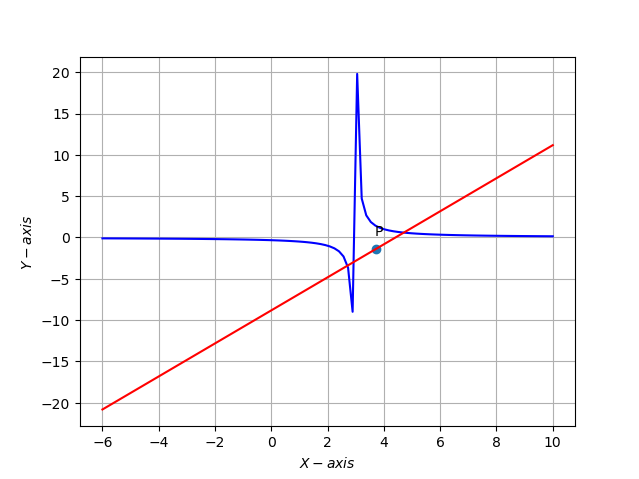
\includegraphics[width=\columnwidth]{chapters/12/6/3/11/figs/con_fig.png}
		\caption{}
		\label{fig:12/6/3/11}
  	\end{figure}
	\iffalse
%\begin{figure}[h]
\vspace{0.25cm}
\includegraphics[width=0.45\textwidth]{con fig.png}\\
\centering{Fig 1. Curve}
\label{fig:circle_1}
%\end{figure}

 \section*{Construction}
 
See Fig 1 for the input parameters in Table 1.\\
\vspace{0.5cm}
{\setlength\extrarowheight{2pt}
\begin{tabular}{|c|c|c|}
	\hline
	\textbf{Symbol}&\textbf{Value}&\textbf{Description}\\
	\hline
	C & $y = \frac{1}{x-3}$ & Given Conic C\\
	\hline
	P & $x_i = q + \mu_i m$ & Point of Contact P\\
	\hline
\end{tabular}
}\\
\vspace{0.25cm}
\centering {Table 1}\\
\section{Solution}
\begin{flushleft}
The equation of  a conic with directrix $\vec{n}^{\top}\vec{x} = c$, eccentricity $e$ and focus $\vec{F}$ is given by 
\end{flushleft}
\begin{align}
    \vec{x}^{\top}\vec{V}\vec{x}+2\vec{u}^{\top}\vec{x}+f=0
\end{align}    

\hspace{-6.5cm}Given, 
\fi
From the given information
\begin{align}
	\vec{V}
	&=\myvec{
		0 &\frac{1}{2}\\\frac{1}{2} & 0\\
	},
\vec{u} = \myvec{
0 \\-\frac{3}{2}
},  f = -1, m=2
	\label{12/6/3/11/eq1}
	\\
	\implies
	\vec{n}&=\myvec{
-m \\ 1 
} = \myvec{-2 \\ 1}  \\
\label{12/6/3/11/eq2}
\end{align}
Hence, the given curve is a hyperbola.
\iffalse
Since
\begin{align}
	\vec{q}&=\vec{V}^{-1}(k_i\vec{n}-\vec{u})    \\
	k_i&=\pm \sqrt{\frac{f_0}{\vec{n}^{\top}\vec{V}^{-1}\vec{n}}}     
\label{12/6/3/11/eq3}
\\
	f_0&=f+\vec{u}^{\top}\vec{V}^{-1}\vec{u}     
\label{12/6/3/11/eq4}
\end{align}
\centering
\begin{align}
n= 
\end{align}
\vspace{0.30cm}
\raggedright
substituting  \eqref{12/6/3/11/eq1} in  \eqref{12/6/3/11/eq4},
\centering
$f_o=-1+\myvec{0 & \frac{-3}{2}}\myvec{0 & 2 \\ 2 & 0}\myvec{0 \\ \frac{-3}{2}}$\\
$f_o=-1+\myvec{0 & \frac{-3}{2}}\myvec{-3 \\ 0}$\\
$f_o=-1+0$\\
\vspace{0.30cm}
\begin{align}
f_0=-1           
\label{12/6/3/11/eq6}
\end{align}
\fi
%\raggedright
Substituting  numerical values, we obtain the condition in 
	\eqref{prop:conic-p-contact-nonparab-cond},
\iffalse
\centering
\vspace{0.3cm}
$k_i=\pm{\sqrt{\frac{-1}{\myvec{-2 & 1}\myvec{0 & 2 \\ 2 & 0}\myvec{-2 \\ 1}}}}$\\
\vspace{0.25cm}
\begin{align}
k_i
=\pm{\sqrt{\frac{-1}{\myvec{ 2 & -4}\myvec{ -2 \\ 1}}}}$\\
\end{align}
\vspace{0.25cm}
\begin{align}
k_i=\pm{\sqrt{-\frac{1}{8}}}   
\label{12/6/3/11/eq7}
\end{align}
\fi
which implies that the line with slope 2 is not a tangent.  This can be verified from Fig. 
		\ref{fig:12/6/3/11}.
\iffalse
\vspace{0.3cm}            
\raggedright
Substituting  \eqref{12/6/3/11/eq7} in \eqref{12/6/3/11/eq2},
\vspace{0.4cm}
\centering
\begin{align}
	\vec{q}&=\myvec{0 & 2 \\ 2 & 0}\brak{\pm{\sqrt{\frac{1}{8}}}\myvec{ -2 \\ 1}-\myvec{0 \\ \frac{-3}{2}}}
	&=\myvec{3.707\\-1.414}
\label{12/6/3/11/eq8}
\end{align}
\raggedright
We know that,\\
\vspace{0.3cm}
\begin{align}
\mu_i=\frac{1}{\vec{m}^{\top}\vec{Vm}}(-\vec{m}^{\top}(\vec{Vq}+\vec{u})
\end{align}
\begin{align}
\pm\sqrt{(\vec{m}^{\top}(\vec{Vq+u}))^2-(\vec{q}^{\top}+2\vec{u}^{\top}\vec{q}+f)(\vec{m}^{\top}\vec{Vm})}                 
\label{12/6/3/11/eq9}
\end{align}
%\fi
 substituting Eq. \eqref{12/6/3/11/eq1} and \eqref{12/6/3/11/eq8} in 
\eqref{eq:tangent_roots},
\begin{align}
\mu_i = 0
\label{12/6/3/11/eq10}
\end{align}
Now the point of contact is given by,\\
	\label{eq:chord-pts}
\begin{align}
\vec{x_i = q+\mu_im}
\label{12/6/3/11/eq11}
\end{align}
By substituting Eq. \eqref{12/6/3/11/eq8} and \eqref{12/6/3/11/eq10} in Eq. \eqref{12/6/3/11/eq11} we get,\\
\vspace{0.5cm}
\centering
$P = \myvec{3.707\\-1.414}$\\
\vspace{1cm}
\raggedright
But when we plot the tangent through this point P with the given slope 2, we observe that it touches the curve at 2 points.\\
\vspace{0.5cm}
Hence tangents are not possible for the given curve with slope 2.\\  
\end{document}
\fi
